% This is the magic command for latextools(ST3)
%! TEX program = latexmk -xelatex
\XeTeXgenerateactualtext=1

%%%%%%%%%%%%%% 文字コードについて %%%%%%%%%%%%%%
% Windows では標準で文字コードが Shift-JIS に  %
% である事が多いが,TeX のソースコードは UTF-8 %
% 書くことを推奨する                           %
%%%%%%%%%%%%%%%%%%%%%%%%%%%%%%%%%%%%%%%%%%%%%%%%

% 行頭に '%' をつけるとコメントになる

%%% ドキュメントクラスの設定 %%%
% 基本的にここは変更しない
% 文章全体の文字サイズを変えたい場合は 'XXpt' を変更すること
% デフォルトの文字サイズは10pt
\documentclass[a4paper, twocolumn, xelatex, 9pt, ja=standard, Ligatures=TeX]{bxjsarticle}

%%% プレアンブル ---ここから %%%

% Preamble.tex のインポート
% This is the magic command for latextools(ST3)
%!TEX root = ./Report.tex

%%%%%%%%%%%%%%%%%%%%%%%%%%%%%%%%%%%%%%%%%%%%%%
%%%%%%%%%%%%%%%  各種設定  %%%%%%%%%%%%%%%%%%%
%%%%%%%%%%%%%%%%%%%%%%%%%%%%%%%%%%%%%%%%%%%%%%

\setpagelayout{top=20truemm, bottom=20truemm, left=12truemm, right=12truemm}

\usepackage{xeCJK}
\usepackage{graphicx}
\usepackage{xcolor, color}
\usepackage{here}
\usepackage{ascmac}
\usepackage[hyphens]{url}
\urlstyle{tt}

%%%%%%%%%%%%%%%%%%%%%%%%%%%
%%% フォント指定(XeTeX) %%%
%%%%%%%%%%%%%%%%%%%%%%%%%%%

%% 1. macOS ユーザー向け設定
%% Hiragino, Helvetica, TimesNewRoman, RictyDiminishedDiscord  
	% \usepackage{fontspec}
	% % serifフォント(日本語)
	% \setCJKmainfont[BoldFont={HiraginoSans-W6}]{HiraMinProN-W3}
	% % sans-serifフォント(日本語)
	% \setCJKsansfont[BoldFont={HiraginoSans-W6}]{HiraginoSans-W3}
	% % serifフォント(欧文)
	% \setmainfont[ItalicFont={HelveticaNeue-LightItalic}, BoldFont={HelveticaNeue-Medium}, BoldItalicFont={HelveticaNeue-MediumItalic}]{TimesNewRomanPSMT}
	% % sans-serifフォント(欧文)
	% \setsansfont[ItalicFont={HelveticaNeue-LightItalic}, BoldFont={HelveticaNeue-Medium}, BoldItalicFont={HelveticaNeue-MediumItalic}]{HelveticaNeue-Light}

	% \setmonofont[ItalicFont={RictyDiminishedDiscord-Oblique}, BoldFont={RictyDiminishedDiscord-Bold}, BoldItalicFont={RictyDiminishedDiscord-BoldOblique}]{RictyDiminishedDiscord-Regular}
	% \setCJKmonofont[ItalicFont={RictyDiminishedDiscord-Oblique}, BoldFont={RictyDiminishedDiscord-Bold}, BoldItalicFont={RictyDiminishedDiscord-BoldOblique}]{RictyDiminishedDiscord-Regular}

% 2. NotoSansCJKjp、NotoSerifCJKjp、NotoSans、NotoSerif、RictyDiminishedDiscord
	\usepackage{fontspec}
	% serifフォント(日本語)
	\setCJKmainfont[BoldFont={NotoSansCJKjp-Medium}]{NotoSerifCJKjp-Light}
	% sans-serifフォント(日本語)
	\setCJKsansfont[BoldFont={NotoSansCJKjp-Medium}]{NotoSansCJKjp-Light}
	% serifフォント(欧文)
	\setmainfont[ItalicFont={NotoSerif-LightItalic}, BoldFont={NotoSerif-Medium}, BoldItalicFont={NotoSerif-MediumItalic}]{NotoSerif-Light}
	% sans-serifフォント(欧文)
	\setsansfont[ItalicFont={NotoSans-LightItalic}, BoldFont={NotoSans-Medium}, BoldItalicFont={NotoSans-MediumItalic}]{NotoSans-Light}

	\setmonofont[ItalicFont={RictyDiminishedDiscord-Oblique}, BoldFont={RictyDiminishedDiscord-Bold}, BoldItalicFont={RictyDiminishedDiscord-BoldOblique}]{RictyDiminishedDiscord-Regular}
	\setCJKmonofont[ItalicFont={RictyDiminishedDiscord-Oblique}, BoldFont={RictyDiminishedDiscord-Bold}, BoldItalicFont={RictyDiminishedDiscord-BoldOblique}]{RictyDiminishedDiscord-Regular}


% 日付フォーマット変更
\renewcommand{\today}{\the\year/\the\month/\the\day}

% \maketitle カスタマイズ
\usepackage{titling}
\pretitle{
	\vspace{-2.3cm} % タイトルを上に詰める
	\begin{center}
		\huge\sffamily % タイトル:hugeサイズ、ゴシック体
}
\posttitle{
	\end{center}
}
\preauthor{
	\vspace{\baselineskip}
	\begin{center}
		\large\sffamily % 著者名:largeサイズ、ゴシック体
}
\postauthor{
	\end{center}
}
\predate{
	\begin{center}
		\large\sffamily % 日付:largeサイズ、ゴシック体
}
\postdate{
	\end{center}
}


% セクションのスタイル変更
\usepackage{titlesec}
\titleformat*{\section}{\Large\bfseries\sffamily}
\titleformat*{\subsection}{\normalsize\bfseries\sffamily}


% 参照マクロ
\newcommand{\fref}[1]{\textbf{図\ref{#1}}}
\newcommand{\Fref}[1]{\textbf{式\ref{#1}}}
\newcommand{\tref}[1]{\textbf{表\ref{#1}}}


% listings 設定
% listings: ソースコードを表示するためのプラグイン
\usepackage{listings}

% コード部分の色スタイルの設定
\definecolor{bkg}{gray}{0.95}
\definecolor{def}{gray}{0.00}
\definecolor{com}{gray}{0.60}
\definecolor{key}{rgb}{0.00, 0.00, 0.75}
\definecolor{str}{rgb}{0.20, 0.50, 0.15}

% ソースコードを表示するときのキャプション名
\renewcommand{\lstlistingname}{コード}

% 書式設定
\lstset{
   % プログラミング言語
   language={C},
   % 背景色
   backgroundcolor={\color{bkg}},
   % 基本の文字スタイル
   basicstyle={\small\ttfamily\color{def}},
   % 変数の文字スタイル
   identifierstyle={\small\ttfamily\color{def}},
   % コメントの文字スタイル
   commentstyle={\color{com}},
   % 予約語の文字スタイル
   keywordstyle={\bfseries\color{key}},
   % 非予約語の文字スタイル (よくわからない)
   ndkeywordstyle={\small\color{def}},
   % 文字列リテラルのスタイル
   stringstyle={\bfseries\color{str}},
   % 枠線の設定
   % t, r, b, l: それぞれ上、右、下、左の1本線
   % T, R, B, L: それぞれ上、右、下、左の2本線
   frame={tlRB},
   % 長い文を改行するかどうか
   breaklines=true,
   % 横幅間隔の調整
   columns=[l]{fullflexible},
   % 左右のマージン
	 xrightmargin=0\zw,
   xleftmargin=1\zw,
   framexleftmargin=3pt,
   % 行番号の位置
   numbers=left,
   % 行番号のスタイル
   numberstyle={\ttfamily\small},
   % 行番号とコード本文の間の空白
	 numbersep=1\zw,
   % 行番号の刻み
   stepnumber=1,
   % コメント行の継続の設定
	morecomment=[l]{//}
}
\newcommand{\cref}[1]{\textbf{\lstlistingname\ref{#1}}}


% 行間隔の変更 (0.90倍に)
% \renewcommand{\baselinestretch}{0.90}

%%% プレアンブル ---ここまで %%%

%%% タイトル,筆者,日付の設定 %%%
\title{\vspace{-1cm}\LARGE ドローン空撮映像を用いた災害領域検出}
\author{\vspace{-1cm}静岡大学\ 情報学部\ 佐治研究室 \\ 7071-0090\ 室永\ 将門}
\date{}
% 文字としての空白を入れるときは,
% '\ ' (バックスラッシュ + 半角スペース)
% を入力する


%%%%%%%%%%%%%%%%%%%%%%%%%%%%%%%%%%%%%%%%%%%%%%
%%%%%%%%%%%%%%%%  本文 部分  %%%%%%%%%%%%%%%%%
%%%%%%%%%%%%%%%%%%%%%%%%%%%%%%%%%%%%%%%%%%%%%%

% インデントは必須ではないが,可読性のために
% インデントを推奨する

\begin{document}	
\maketitle
\section{はじめに}
	近年,豪雨による斜面崩壊・浸水被害が多発し,これらの被害箇所を早急に把握することは救助・復旧・二次災害の防止等に有効である.この災害把握に関し,安全な位置からの解析が可能なリモートセンシング技術が注目されている.\\
	リモートセンシング技術による災害領域検出には主に人工衛星,有人航空機(以下,ヘリコプター),無人航空機(以下,ドローン)が用いられる.人工衛星は広範囲の把握が可能であり,画像処理において扱いが容易な直下視点の画像が得られるが,解像度が低く,天候や撮影周期によっては画像が得られないことがある.ヘリコプターは人工衛星に比べ早期に画像を取得でき,解像度が高いが,金銭的コストが非常に高く,周囲に発着場が必要である.これに対しドローンは安価かつ迅速に解像度の高い画像の取得が可能であるため,被害箇所の早急な把握に有効である.江口ら\cite{art01}は災害後の人工衛星画像を用いて斜面崩壊領域を検出する手法を提案しているが,解像度が低く人工物を誤検出するという問題がある.中山\cite{art02}らは災害後のヘリコプター空撮画像を用いて斜面崩壊領域を検出する手法を提案しているが,人工物誤検出低減のためのDEMとの位置合わせの際にずれが生じるという問題がある.雨宮\cite{art03}らは災害後のヘリコプター空撮画像を用いて浸水領域を検出する手法を提案しているが,建物データ等を用いても建物領域の除去精度が低いという問題がある.
	以上を踏まえ,本研究では補助データを用いずに誤検出を抑え,災害後のドローン空撮画像を用いた斜面崩壊・浸水領域を検出する手法を提案する.

\section{提案手法}
	提案手法の概要図を\fref{img01}に示す.提案手法ではドローン空撮映像を分割したフレーム画像を入力画像とし,災害領域検出結果より不要領域検出結果を除去した斜面崩壊・浸水領域の検出結果を出力画像とする.
	
\begin{figure}[b]
	\centering
		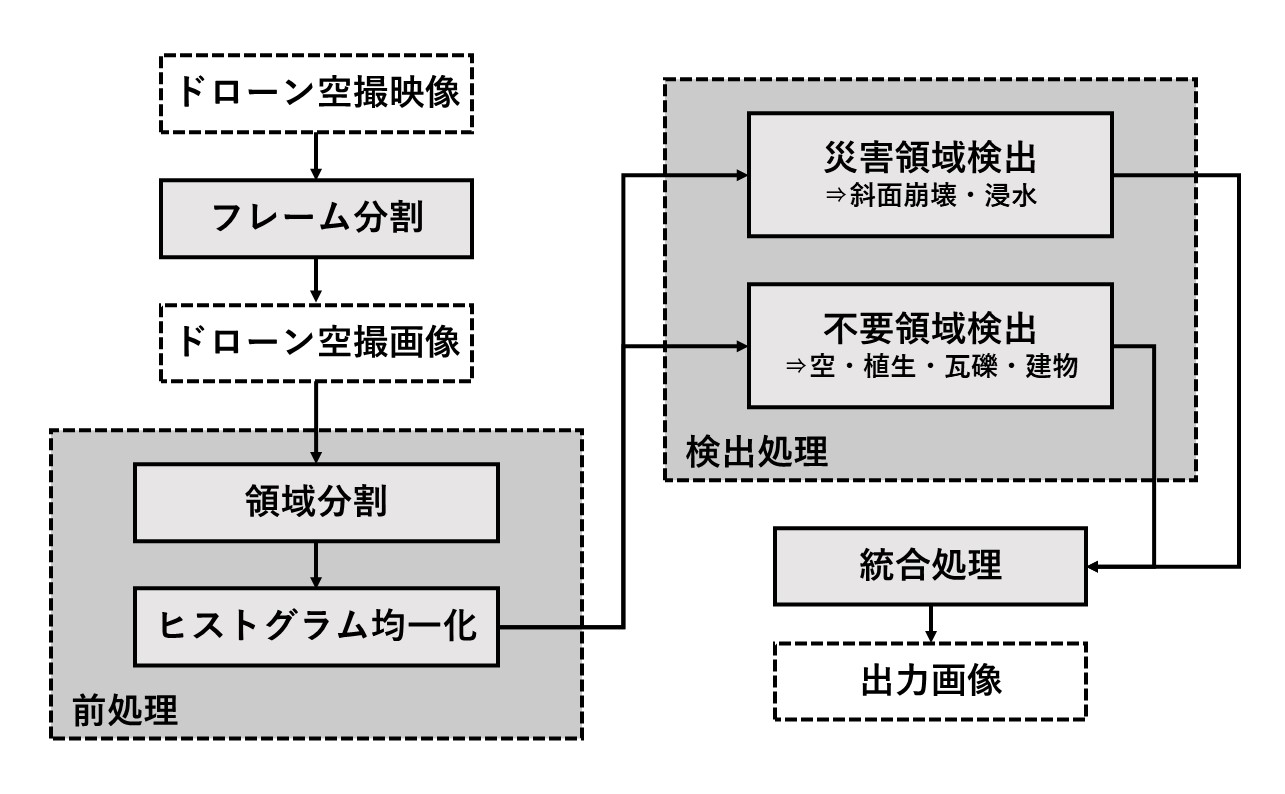
\includegraphics[width=8cm]{img/howto.jpg}
		\caption{提案手法概要図}
		\label{img01}
\end{figure}

\subsection{領域分割}
	本研究では領域ごとに斜面崩壊・浸水領域を判別するため,フレーム画像に対しMean-Shift法による領域分割を行う.Mean-Shift法を用いると近傍の類似した色相を持つ画素郡を同一色に統合し,同一の領域として扱うことができる.

\subsection{ヒストグラム均一化}
	空撮画像は撮影時の天候や時刻によって色相や輝度に偏りが生じるため,CLAHEのアルゴリズムによって領域分割処理後画像に対しヒストグラム均一化を行う.CLAHEのアルゴリズムは画像を小領域に分割し,小領域毎にヒストグラム平坦化を行う手法で,空撮画像特有の偏りを低減する効果がある.
	
\subsection{災害領域検出}
	各災害領域の特徴を\tref{tab01}に示す.これら色相等の特徴を用いて各領域の検出を行う.

	\begin{table}[h]
		\centering
		\caption{各災害領域の特徴}
		\label{tab01}
		\begin{tabular}{c c c c c}
			\hline
			領域名 & 色相 & 彩度 & 輝度 & 均一度 \\
			\hline
			\hline
			斜面崩壊 & 赤 & 高 & 低 & -- \\
			浸水 & 赤 & 低 & 高 & 高 \\ \hline
		\end{tabular}
	\end{table}

	\subsubsection{斜面崩壊領域}
		斜面崩壊領域は色相と輝度,彩度にて検出を行うためL*a*b*表色系のL*値,a*値とHSV表色系のS値を用いる.L*a*b*表色系は人間の視覚に近い色空間であり色相による分類に有効である.L*値は輝度を表し,赤い画素ではa*値が高く,青い画素と緑の画素ではそれぞれb*値とa*値が低い.HSV表色系は色相,彩度,明度の情報を持つ色空間でありこれらの特徴を利用する場合に用いられる.本研究では彩度を表すS値を用いる.ヒストグラム均一化処理後の画像に対しL*a*b*表色系変換とHSV表色系変換を行い,これらの指標を用いた閾値処理により斜面崩壊領域を検出する.
		
		% なお,L*a*b*表色系は人間の		
		% これらの指標による閾値処理にて斜面崩壊領域を検出する.
		% 斜面崩壊領域はL*a*b*表色系のa*値,L*値とHSV表色系のS値が低いという特徴がある.a*値が高いとき赤が強く,L*値とS値は輝度と彩度を表す.	これらの特徴を用いて閾値処理を行う.
	\subsubsection{浸水領域}
		前項同様にL*値,a*値,S値を用いる.また,浸水領域は表面が均一であるためエッジがほとんど存在しないためフレーム画像よりCanny法にてエッジを検出し,領域単位でエッジ抽出率を算出する.色相等の指標と領域単位でのエッジ抽出率による閾値処理によって浸水領域を検出する.

\subsection{不要領域検出}
	各不要領域の特徴を\tref{tab02}に示す.前節と同様にこれらの特徴を用いて各領域の検出を行う.
	
	\begin{table}[h]
		\centering
		\caption{各不要領域の特徴}
		\label{tab02}
		\begin{tabular}{c c c c c}
			\hline
			領域名 & 色相 & 彩度 & 輝度 & 均一度 \\
			\hline
			\hline
			空 & 青 & -- & 高 & -- \\
			植生 & 緑 & -- & -- & -- \\
			瓦礫 & -- & -- & -- & 低 \\
			建物 & -- & -- & -- & 高 \\ \hline
		\end{tabular}
	\end{table}

\subsubsection{空領域}
	ドローンは撮影視点が横方向となることが多く画像中に空領域を含むことがあるため,空領域を除去することで誤検出を低減する.前節同様にL*値とb*値を用いた閾値処理によって空領域を検出する.
	
	% 空領域はb*値が低く,L*値が高いという特徴があるため閾値処理によって検出を行う.なお,b*値が低いとき青が強くなる.
\subsubsection{植生領域}
	山間部では画像中に多量の植生領域を含むため,植生領域を除去する.前節同様にa*値を用いた閾値処理によって植生領域を検出する.
	
	% 植生領域はa*値が低いという特徴があるため閾値処理によって検出を行う.
\subsubsection{瓦礫領域}
	瓦礫領域は災害領域と色相が類似しており本研究の災害領域検出手法では誤検出を起こしやすいため除去する.瓦礫領域は多量のエッジを含むため前節と同様にエッジ抽出率を算出し,抽出率が高い領域を瓦礫領域とする.

	% 斜面崩壊,浸水,人工物領域は色相が類似していることが多く,2.4節のような色特徴での除去が難しい.そこで,本研究ではテクスチャ特徴量の指標の一つである異質度にて閾値処理を行う.異質度とは画像内の不均一度を示す指標であり,表面が不均一である程高い値を示す.
\subsubsection{建物領域}
	建物領域は災害領域と色相が類似していることが多く誤検出を起こしやすいため除去する.建物領域の屋根や壁は均一度が高いため表面粒径サイズが大きいほど高い値を示すGSI(Grain Size Index)を領域単位で算出し,GSIが閾値より低い画素の多い領域を建物領域とする.また,R,G,BをRGB表色系の各値としてGSIのの算出式を以下に示す.

	\begin{equation}
		GSI = \frac{R-B}{R+B+G}
	\end{equation}

	% 建物領域は建物ごとに色相が異なるため色相による分類が難しい.よって,本研究では画像表面の均一度を示すGSI(Grain Size Index)という指標を用いる.

\section{実験}
\subsection{実験結果}
	本実験では平成29年7月九州北部豪雨のドローン空撮映像\cite{web01}を用いた.\tref{tab03}に空撮映像の詳細を示す.また,\fref{img02}--\fref{img06}に入力画像と各処理の出力画像を示す.
\subsection{精度評価}
	目視判読により斜面崩壊・浸水領域の正解画像を手動で作成し,画素単位での適合率,再現率,F値にて精度評価を行った。作成した正解画像と精度評価結果を\fref{img08}と\tref{tab04}に示す。

	\begin{table}[h]
		\centering
		\caption{実験データ}
		\label{tab03}
		\begin{tabular}{l l}
			\hline
			災害名称 & 平成29年7月九州北部豪雨 \\
			撮影箇所 & 福岡県朝倉市赤谷川 \\
			撮影日時 & 平成29年7月7日15時30分 \\
			解像度 & 1920 × 1080 pixel \\
			提供 & 国土地理院 \\ \hline
		\end{tabular}
	\end{table}
	
	\begin{figure}[b]
		\begin{minipage}{0.48\hsize}
			\centering
			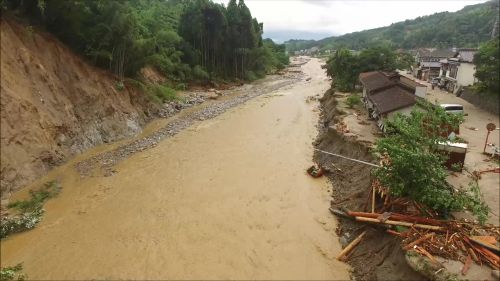
\includegraphics[width=\linewidth]{img/original.png}
			\caption{入力画像}
			\label{img02}
		\end{minipage}
		\begin{minipage}{0.48\hsize}
			\centering
			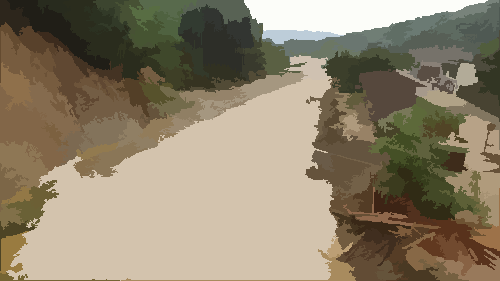
\includegraphics[width=\linewidth]{img/meanshift.png}
			\caption{領域分割}
			\label{img03}
		\end{minipage}
	\end{figure}
	\begin{figure}[t]
		\begin{minipage}{0.48\hsize}
			\centering
			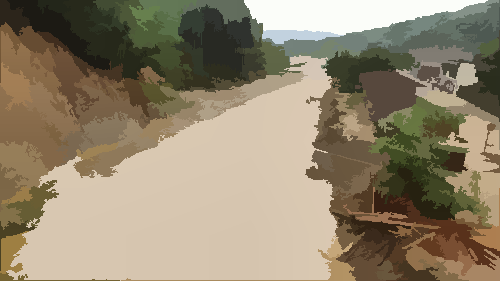
\includegraphics[width=\linewidth]{img/equalization.png}
			\caption{ヒストグラム均一化}
			\label{img04}
		\end{minipage}
		\begin{minipage}{0.48\hsize}
			\centering
			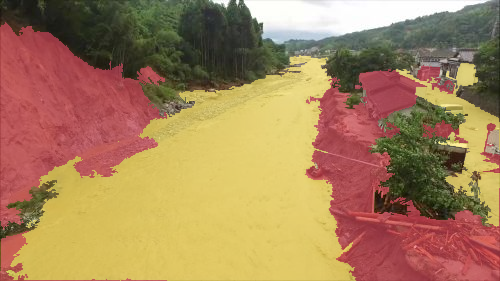
\includegraphics[width=\linewidth]{img/detection.png}
			\caption{災害領域検出(赤:斜面崩壊,黃:浸水)}
			\label{img05}
		\end{minipage}
	\end{figure}
	\begin{figure}[t]
		\begin{minipage}{0.48\hsize}
			\centering
			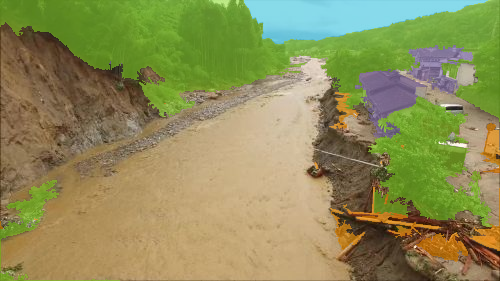
\includegraphics[width=\linewidth]{img/rejection.png}
			\caption{不要領域検出(青:空,緑:植生,橙:瓦礫,紫:建物)}
			\label{img06}
		\end{minipage}
		\begin{minipage}{0.48\hsize}
			\centering
			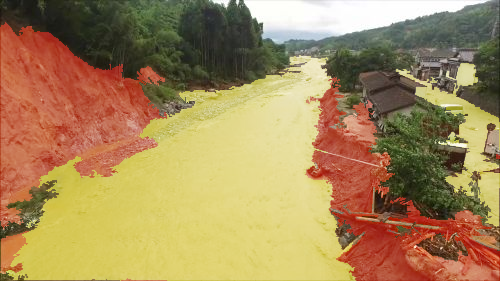
\includegraphics[width=\linewidth]{img/result.png}
			\caption{出力画像(赤:斜面崩壊,黃:浸水)}
			\label{img07}
		\end{minipage}
	\end{figure}
	\begin{figure}[t]
		\begin{minipage}{0.48\hsize}
			\centering
			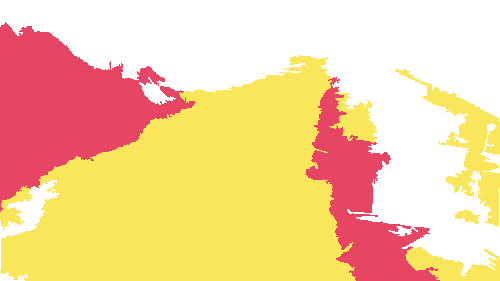
\includegraphics[width=\linewidth]{img/answer.png}
			\caption{正解画像(赤:斜面崩壊,黄:浸水)}
			\label{img08}
		\end{minipage}
	\end{figure}

	\begin{table}[h]
		\centering
		\caption{精度評価}
		\label{tab04}
		\begin{tabular}{c c c c}
			\hline
				実験 & 再現率 & 適合率 & F値 \\ \hline
				斜面崩壊領域 & 0.953 & 0.596 & 0.733 \\
				浸水領域 & 0.848 & 0.987 & 0.912 \\ \hline
		\end{tabular}
	\end{table}

\section{まとめ・今後の予定}
	本実験ではドローン空撮映像から斜面崩壊・浸水領域を検出する手法を提案した.現状の問題点として瓦礫領域除去の際に斜面崩壊領域を除去してしまう点や,斜面崩壊・浸水領域同士の誤検出が起きる点が挙げられる.また,浸水領域に関し,既存の河川と災害によって水没した浸水箇所の判別は未実装である.\\
	 今後はこれらの誤検出改善・実装を進め,システムの精度向上を目指す.

\section{参考文献}		
	% 参考文献はbibtexを用いて作成する.文献を参照するには\cite{鈴木:論文06},\cite{Web01}とする.

% 参考文献の表示
\bibliographystyle{junsrt}   % 参考文献の並び順を指定
\bibliography{bib/myref.bib} % \bibliography{参考文献ファイルへのパス}

\end{document}
